\subsection{协议实现细节}
\label{subsec:implementation_details}

协议实现采用“分层抽象,组件解耦”的设计理念,构建了一个既安全又灵活的实现框架。

\subsubsection{参与方角色与职责}

\textbf{客户端(C)} 作为协议的发起方,负责启动会话建立过程,无需持有预先验证的身份或长期密钥,可以匿名参与协议,简化身份管理并提高隐私性。主要职责包括生成临时密钥对、使用服务器公钥封装共享密钥、派生会话密钥以及发送可选的0-RTT加密数据。客户端实体封装了完整的协议状态机和会话管理逻辑,提供简洁的API,如GenerateClientHello()和ProcessServerResponse(),使应用层代码能够轻松集成协议功能,无需了解底层细节。

\textbf{服务器(S)} 作为协议的响应方,持有长期密钥对,需要通过某种可信机制(如证书机构)将其公钥分发给客户端,负责验证客户端请求、解封装共享密钥、派生会话密钥,并通过成功解密客户端消息来隐式完成身份认证。在第二阶段,服务器还负责使用客户端临时公钥封装共享密钥,建立具有弱前向安全性的主会话密钥。协议采用单边认证,只对服务器进行身份认证,客户端可以匿名参与,该模式适用于许多实际场景,如Web浏览器与HTTPS服务器的通信通常仅验证服务器身份,而客户端身份的验证作为可选项。

\label{subsubsec:system_architecture}
系统采用分层架构和模块化设计,各功能组件高度解耦,提高代码可维护性、可测试性和可扩展性,整体架构包含五个核心层次,如图\ref{fig:system-architecture}所示:

\textbf{应用层}作为系统的最外层,面向用户提供协议交互的高级抽象,封装了客户端和服务器实体以及完整的消息交换流程,使开发者无需了解底层密码学细节即可使用协议。应用层还实现了完整的0-RTT数据传输功能,允许客户端在首个往返中发送加密数据,大大减少了通信建立的延迟。

\textbf{序列化层}负责协议消息的编码与解码,确保跨平台通信的一致性。该层定义了ClientHello和ServerResponse消息的二进制格式和处理逻辑,采用长度前缀编码方式,确保调用对应功能函数能正确解析报文。

\textbf{协议核心层}是系统的主要中枢,实现了状态管理、会话处理和密钥协商逻辑,采用状态机模式,将协议分为初始、等待响应、已建立和失败四个主要状态,通过状态转换规则确保协议执行的正确性。核心层定义了统一的会话接口,隔离了客户端和服务器的具体实现差异,使上层应用能够以一致的方式操作会话,无须区分对应角色。

\textbf{KEM接口层}是TIMKE实现的关键创新之一,通过定义统一的KEM操作接口,实现了协议与具体KEM算法的解耦,灵活适配不同的后量子KEM实现,不仅支持自实现的OW-ChCCA KEM,还能无缝集成ML-KEM等标准算法。通过注册表模式和工厂模式的结合,支持运行时的KEM算法选择,用户可以根据安全需求和性能考量选择最适合的KEM组合。

\textbf{加密原语层}作为系统的基础,提供哈希函数、对称加密等操作,封装底层密码库的具体实现细节,为上层提供统一的安全原语接口。密钥派生功能的实现基于SHA3的哈希链,确保会话密钥的安全性和唯一性。对称加密组件支持用户自行更换,实现采用AES-GCM模式,同时提供保密性和完整性保护。

系统架构如图\ref{fig:system-architecture}所示,展示各组件之间的关系和数据流。架构遵循关注点分离原则,使各组件能够独立演化和测试,可以在不修改协议核心逻辑的情况下,替换KEM算法实现或更新序列化方式,同时也便于进行单元测试和性能优化,为协议的长期维护和演进奠定基础。

\begin{figure}[ht]
  \centering
  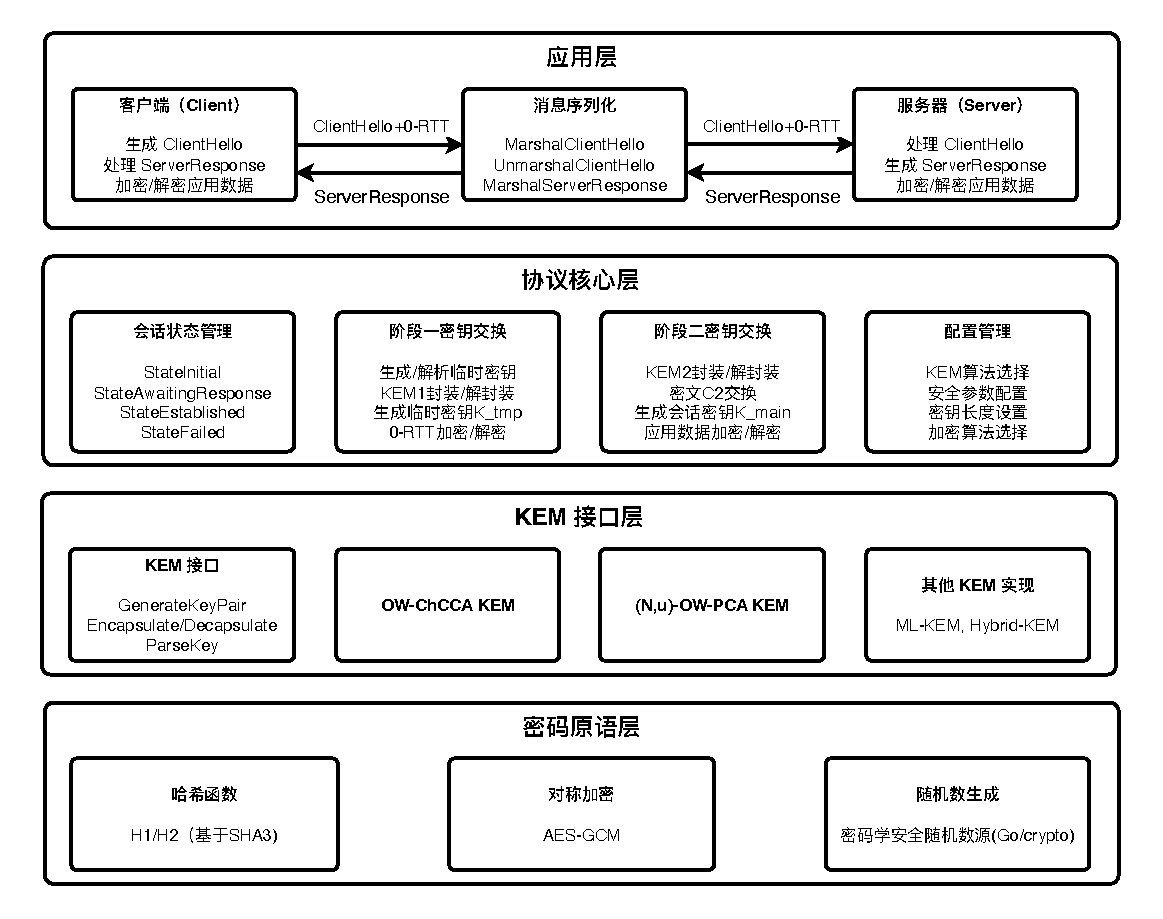
\includegraphics[width=\textwidth]{doc/graph/implementation.drawio.pdf}
  \caption{TIMKE协议实现架构}
  \label{fig:system-architecture}
\end{figure}


\subsubsection{KEM集成与灵活配置}
\label{subsubsec:kem_implementation}
TIMKE协议要求两种不同安全特性的KEM组件:KEM\textsubscript{1}需满足OW-ChCCA安全,KEM\textsubscript{2}需满足OW-PCA安全。

KEM\textsubscript{1}使用第\ref{chap:owchccakem}章详述的自实现OW-ChCCA KEM,该实现遵循理论构造,满足紧致安全。考虑到OW-ChCCA KEM在性能上的局限性,实现也支持使用更高效的ML-KEM作为替代方案,虽然在理论上削弱了紧致安全的保证,但在实际测试中有更好的性能表现。

KEM\textsubscript{2}使用具有更强安全性(IND-CCA2)的KEM方案,主要采用Cloudflare的CIRCL\cite{circl}库提供的后量子KEM实现,它们具有足够的强的安全性和性能表现,许多现代加密应用都基于此库进行设计。

KEM接口层是TIMKE协议实现的核心之一,定义协议与具体KEM算法交互的标准方式,支持多种KEM算法,从而满足不同的安全需求和计算环境约束,还定义了标准的操作集,包括密钥生成、封装、解封装等功能,如代码\ref{code:kem-interface}所示:

\begin{listing}[ht]
\begin{minted}{go}
type KEM interface {
    // 返回KEM的参数信息
    Setup() Parameters
    // 生成密钥对
    GenerateKeyPair(params Parameters, rand io.Reader) (PublicKey, PrivateKey, error)
    // 使用公钥封装共享密钥
    Encapsulate(pk PublicKey, rand io.Reader) (ciphertext []byte, sharedSecret []byte, err error)
    // 使用私钥解封装共享密钥
    Decapsulate(sk PrivateKey, ciphertext []byte) ([]byte, error)
    // 解析二进制格式的公钥
    ParsePublicKey(data []byte) (PublicKey, error)
    // 解析二进制格式的私钥
    ParsePrivateKey(data []byte) (PrivateKey, error)
}
\end{minted}
\caption{KEM接口定义}
\label{code:kem-interface}
\end{listing}

接口设计充分考虑了现代密码库的实践经验,提供了完整的生命周期管理和错误处理,确保协议能够安全处理各种边缘情况和异常状态。接口的rand io.Reader参数允许注入不同的随机源,便于测试和安全审计,而可选的params参数则支持不同安全级别的参数配置。

为支持TIMKE协议实现的长期可维护性和算法更新能力,实现在此接口的基础上设计了完整的KEM注册与动态配置模块。该模块基于工厂模式和注册表模式的组合实现,允许在运行时根据名称动态选择KEM算法,维护算法名称到实现构造函数的映射,支持列举可用算法、获取算法实例和动态注册新算法,还支持算法优先级排序和默认算法配置,在特定算法不可用时自动选择合适的替代方案。实现预注册包括OW-ChCCA KEM、ML-KEM等在内的多种算法,并为用户提供清晰的接口以添加自定义实现,具体包括:

\begin{enumerate}
    \item \textbf{OW-ChCCA KEM}:基于格密码实现的单向可检测选择密文安全KEM,对应协议安全证明,实现了多个安全级别,满足不同强度需求。
    
    \item \textbf{后量子KEM}:集成了主流的后量子安全KEM算法:
    \begin{itemize}
        \item \textbf{ML-KEM}(FIPS 203标准):支持ML-KEM-512、ML-KEM-768和ML-KEM-1024不同安全级别
        \item \textbf{混合KEM}:如X25519-ML-KEM-768等组合方案,同时提供经典安全和后量子安全
    \end{itemize}
\end{enumerate}

为支持灵活的KEM算法配置,实现采用注册表模式和工厂模式,如代码\ref{code:kem-registry}所示。

\begin{listing}[ht]
\begin{minted}{go}
func init() {
    // 注册OW-ChCCA KEM实现
    RegisterKEM("OWChCCA-64", func() KEM {
        kem, _ := NewOwChCCAKEM(Security64Type)
        return kem
    })
    ...
    // 注册ML-KEM实现
    RegisterKEM("ML-KEM-512", func() KEM {
        kem, _ := NewCirclKEM(MLKEM512Type)
        return kem
    })
    ...
    // 注册混合KEM实现
    RegisterKEM("X25519-ML-KEM-768", func() KEM {
        kem, _ := NewCirclKEM(MLKEM768X25519Type)
        return kem
    })
    // 其他KEM实现注册...
}
\end{minted}
\caption{KEM注册代码}
\label{code:kem-registry}
\end{listing}

\subsubsection{协议状态管理}
\label{subsubsec:state_management}

TIMKE协议涉及复杂的状态转换和会话管理,采用状态机模式进行管理可以清晰界定协议的不同阶段和转换条件。实现定义了四种核心状态,以映射协议的不同阶段:StateInitial为初始状态,表示会话尚未开始;StateAwaitingServerResponse表示客户端已发送请求,正在等待服务器响应;StateEstablished表示会话已成功建立,可以安全通信;StateFailed表示会话建立失败,需要重新协商。

客户端和服务器各自维护独立的状态,通过交互推动相应状态的转换。客户端状态管理涵盖了从会话初始化到密钥建立的完整流程,关注状态转换的正确性与安全性。例如,在初始状态下才能生成ClientHello消息,在等待响应状态下才能处理ServerResponse消息。服务器状态管理侧重于请求处理和响应生成,如临时会话密钥和主会话密钥的派生,需要验证客户端消息的有效性,正确解封装共享密钥并响应。实现中的状态转换会考虑相应错误,如解封装失败、格式错误或超时,并采取相应的恢复策略。代码\ref{code:state-transition}展示了客户端状态转换逻辑:

\begin{listing}[ht]
\begin{minted}{go}
func (c *Client) GenerateClientHello(zeroRTTData []byte) (*ClientHello, error) {
    if c.state != StateInitial {
        return nil, errors.New("client not in initial state")
    }
    // 生成临时密钥对和KEM1封装
    // ...
    c.state = StateAwaitingServerResponse
    return clientHello, nil
}

func (c *Client) ProcessServerResponse(response *ServerResponse) ([]byte, error) {
    if c.state != StateAwaitingServerResponse {
        return nil, errors.New("client not waiting for server response")
    }
    // 处理服务器响应
    // ...
    c.state = StateEstablished
    return plaintext, nil
}
\end{minted}
\caption{客户端状态转换代码}
\label{code:state-transition}
\end{listing}
状态机确保协议操作的顺序性和安全性,防止状态错误导致的安全问题,也提高了系统的鲁棒性和可靠性。每个状态转换都包含完整的错误处理逻辑,确保在异常情况下能够正确回退或终止会话。
\subsubsection{协议消息格式}
\label{subsubsec:message_format}
协议消息格式设计直接影响通信效率、兼容性和可扩展性,采用简洁而灵活的二进制编码方案,平衡传输效率和解析便捷性,适合资源受限环境和跨平台应用。

协议实现主要定义了两种消息类型:ClientHello和ServerResponse,命名参考自现代密钥交换协议(如TLS)一致,便于理解和集成。

\textbf{ClientHello}消息是客户端发送给服务器的第一个消息,包含以下字段:
\begin{itemize}
  \item \textbf{EphemeralPublicKey} ($epk_C$):客户端生成的临时公钥,用于第二阶段的密钥协商
  \item \textbf{Ciphertext1} ($C_1$):服务器公钥$pk_S$封装得到的密文
  \item \textbf{EncryptedPayload} ($C_{payload}$):临时会话密钥$K_{tmp}$加密的0-RTT数据(可选字段)
  \item \textbf{KEM1Type}:指示KEM\textsubscript{1}类型的标识符(可选,用于协商)
  \item \textbf{KEM2Type}:指示KEM\textsubscript{2}类型的标识符(可选,用于协商)
\end{itemize}

KEM类型标识允许客户端和服务器在运行时协商使用的KEM算法,提高协议的灵活性,当双方支持多种KEM实现时,允许用户根据安全需求和性能考量选择合适的算法。

\textbf{ServerResponse}消息是服务器对ClientHello的响应,包含以下字段:

\begin{itemize}
    \item $C_2$:客户端临时公钥$epk_C$封装得到的密文
    \item $C'_{payload}$:主会话密钥$K_{main}$加密的应用数据(可选)
\end{itemize}

实现采用清晰的序列化和反序列化接口,支持不同的编码选项和错误处理策略。消息解析采用边界检查和格式验证,防止格式错误导致的安全问题,如缓冲区溢出或类型混淆攻击。

\subsubsection{密钥派生机制实现}
\label{subsubsec:key_derivation_impl}

密钥派生是TIMKE协议安全性的核心组成部分,将KEM提供的共享密钥转换为会话密钥,并结合会话上下文信息确保密钥的唯一与安全。实现采用SHA3-512哈希函数作为密钥派生函数的基础,并通过域分隔技术确保不同上下文的派生相互独立,分别用于临时会话密钥和主会话密钥的派生:

\begin{listing}[ht]
\begin{minted}{go}
// H1派生临时会话密钥:K_tmp = H1(pk_S, C_1, K_1)
func H1(pkS, c1, k1 []byte) ([]byte, error) {
    if pkS == nil || c1 == nil || k1 == nil {
        return nil, errors.New("invalid input to H1")
    }

    h := NewHash()
    // 添加域分隔标识,增强安全性
    domain := []byte("TIMKE-H1")
    return h.Hash(domain, pkS, c1, k1)
}

// H2派生主会话密钥:K_main = H2(pk_S, epk_C, C_1, C_2, K_1, K_2)
func H2(pkS, epkC, c1, c2, k1, k2 []byte) ([]byte, error) {
    if pkS == nil || epkC == nil || c1 == nil || c2 == nil || k1 == nil || k2 == nil {
        return nil, errors.New("invalid input to H2")
    }

    h := NewHash()
    // 添加域分隔标识,增强安全性
    domain := []byte("TIMKE-H2")
    return h.Hash(domain, pkS, epkC, c1, c2, k1, k2)
}
\end{minted}
\caption{密钥派生函数代码}
\label{code:key-derivation}
\end{listing}

派生函数的设计遵循以下安全原则:
\begin{itemize}
    \item \textbf{域分隔}:添加唯一的前缀标识符("TIMKE-H1"和"TIMKE-H2")以确保不同上下文的哈希值不会冲突,防止潜在的域混淆攻击。
    \item \textbf{全参数输入}:派生函数包含所有相关的协议状态和密钥材料,确保密钥与特定会话和交互紧密绑定,例如,H2函数包含服务器公钥、客户端临时公钥、两个密文和两个共享密钥,通过上下文绑定防止中间人攻击和会话混淆。
    \item \textbf{输入验证}:检查输入参数,确保不会处理无效数据,防止潜在攻击。
    \item \textbf{安全哈希}:SHA3系列哈希函数是最新的密码学哈希标准,具有优异的安全特性和性能表现,能确保足够的安全强度和抗碰撞性。
\end{itemize}

密钥派生需要处理不同格式的数据,序列化层提供统一的转换函数,确保不同类型的数据能够正确转换为所调用哈希函数输入相符的格式。

\paragraph{量子抗性哈希函数比较}
TIMKE协议的安全性在很大程度上依赖于密钥派生函数的密码学强度,实现选择SHA3-512作为基础哈希函数。SHA3作为最新的哈希函数标准,与SHA2有完全不同的内部结构(Keccak海绵结构),被认为具有良好的抗量子计算能力,也是NIST标准中常用的哈希函数。NIST在ML-KEM标准\cite{nist_mlkem_2024}中还提到可扩展输出函数SHAKE128和SHAKE256,SHAKE128提供128位安全性,SHAKE256提供256位安全性,作为SHA3标准的一部分,允许生成任意长度的输出,无需级联多个哈希值或截断输出,适合生成不同长度的密钥材料。在量子计算的背景下,Grover算法可以将对称密码原语的安全性从$n$位降至$n/2$位,为保证128位安全,实际部署至少需要256位的强度以抵抗量子攻击,SHA3-512和SHAKE256均满足这一要求。当前的SHA3-512实现为协议提供了充分的安全保障,同时SHAKE函数作为备选方案可以在特定场景下进一步优化性能和灵活性。

\paragraph{对称加密实现}
TIMKE协议使用派生的会话密钥保护应用数据的保密性和完整性,选择AES-GCM作为对称加密算法,能同时保证数据的机密性和完整性,如代码\ref{code:symmetric-encryption}示。
实现支持多种对称加密算法,用户可以通过实现SymmetricEncryption接口添加自己的加密方案,如ChaCha20-Poly1305或其他认证加密算法,适应不同环境的安全需求和性能约束,在移动设备上优先选择计算效率较高的算法,而在服务器环境中则优先考虑安全性更高的方案。

\subsubsection{错误处理与安全编程}
\label{subsubsec:error_handling}

密码协议的实现需要关注错误处理和异常情况,存在缺陷或边界条件漏判可能导致严重的安全漏洞。实现采用全面的错误处理策略和防御性编程技术,确保安全性和可靠性。
比如,定义具体的错误类型,提供明确的错误信息,同时避免泄露敏感信息,如代码\ref{code:error-types};采用错误封装模式,保留详细错误上下文,同时屏蔽敏感信息,如代码\ref{code:error-wrapping}。系统采用彩色编码的日志输出,区分不同级别的信息,便于问题诊断和安全审计;通过防御性编程技术,在实现中对所有外部输入进行验证,确保程序状态一致性,参考代码\ref{code:defensive-programming}。

\subsubsection{配置与扩展机制}
\label{subsubsec:configurability}
实用的密码协议需要适应不同的应用场景和安全需求,因此配置灵活性和扩展能力也需要重点考量,TIMKE实现提供多层次的配置接口和扩展点,满足各种应用需求。针对协议的拓展性,所有核心组件均通过接口定义,允许替换具体实现,比如通过注册机制管理KEM算法,便于添加新的算法实现。组件之间通过明确的接口交互,减少耦合,协议核心逻辑与具体加密原语分离,支持不同密码库集成。

\begin{itemize}
    \item \textbf{KEM算法配置}:支持多种KEM算法组合,如OWChCCA-64/ML-KEM-768等,用户可根据安全级别和性能需求选择合适组合
    
    \item \textbf{对称加密配置}:支持替换默认的AES-GCM实现,使用其他对称加密算法(如ChaCha20-Poly1305),适应不同平台优化需求
    
    \item \textbf{会话选项配置}:通过SessionOptions接口灵活配置服务器密钥对和会话参数
\end{itemize}

